\documentclass[a4paper, brazil, 12pt , onecolumn]{report}
\usepackage[T1]{fontenc}
\usepackage[utf8]{inputenc}
\usepackage[brazil]{babel}
\usepackage[dvips]{graphicx}
\usepackage{ae}
\usepackage[top=10mm,bottom=15mm,left=12mm,right=12mm]{geometry}
\usepackage{tabularx}
\usepackage{lipsum}
\usepackage{blindtext}
\usepackage{setspace}
\usepackage{color}
\usepackage{fancyhdr}
\usepackage{fancyvrb}
\usepackage{nomencl}
\usepackage{indentfirst}
\usepackage{amsmath}
\usepackage{listings}
\usepackage{subfigure}
\usepackage{xcolor} 
\definecolor{ocre}{RGB}{243,102,25} 
\usepackage{avant} 
\usepackage{mathptmx}
\usepackage{microtype}
\usepackage{makeidx}
\definecolor{almond}{rgb}{0.94, 0.87, 0.8}
\definecolor{blanchedalmond}{rgb}{1.0, 0.92, 0.8}
\usepackage[alf,abnt-etal-text=it,bibjustif, abnt-emphasize=bf, abnt-etal-list=0]{abntcite}
\newcommand{\ew}[1]               {\emph{#1}}
\newcommand{\ns}[1]               {\mbox{#1}}
\newcommand{\sigla}[1]            {\ns{#1}}
\newcommand{\italico}[1]          {\textit{#1}}
\newcommand{\negrito}[1]          {\textbf{#1}}
\newcommand{\subl}[1]             {\underline{#1}}
\newcommand{\cf}[1]               {\texttt{#1}}
\newcommand{\X}{\textbullet}
\newcommand{\Y}{$\circ$}
\renewcommand{\lstlistingname}{\bf Listagem} 

\definecolor{mygreen}{rgb}{0,0.6,0}
\definecolor{mygray}{rgb}{0.5,0.5,0.5}
\definecolor{mymauve}{rgb}{0.58,0,0.82}


\usepackage[Bjarne]{fncychap}
\title{Palestra \LaTeX}
\author{Luciano Senger}
\makeindex
\begin{document}
	\maketitle
	\tableofcontents
	\listoffigures
	\listoftables
\chapter{Introdução}

Hello World!
O parâmetro \cf{alpha} regula a quantidade de tensão no sistema, conforme página \pageref{sec:mat}.
Ele deve ser \textit{escolhido} empiricamente~\footnote{Consultar manual.}.
De acordo com a nacional re \mbox{UTSCA}. 
\subsection{Valores padrão}
O valor padrão é igual a~30 ou~50.
A tensão final será igual $v = \sum_{i=0}^n \frac{x \times y}{\alpha}$, que corresponde ao total.
Conforme equação~\ref{eq:tensao}, pode-se observar que~\ref{fig:alfa}.

\begin{equation}
	v = \sum_{i=0}^n \frac{x \times y}{\alpha}
\end{equation}\label{eq:tensao}

\begin{figure}[htb]
	\centering
	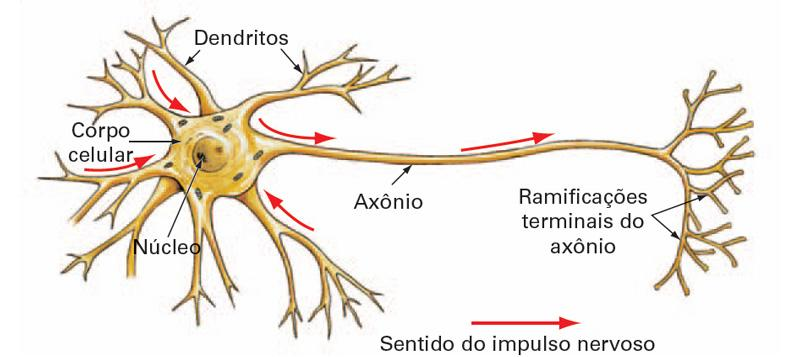
\includegraphics[scale=.1]{neuronio}
	\caption{Mapa mental do \LaTeX}
\end{figure}\label{fig:alfa}

O parâmetro {\Huge \index{beta}} \textbf{regula} a impedância.
Já aprendi 10\% de latex.
As variáveis são:
\begin{itemize}
	\item variavel b;
	\item alpha;
	\item variavel c.
\end{itemize}

\begin{enumerate}
	\item variavel b;
	\item alpha;
	\item variavel c.
\end{enumerate}
A Tabela~\ref{tab:idade} apresenta os valores médio.
\begin{table}[htb]
	\caption{Idade e peso médio observados}\label{tab:idade}
	\centering
	
	\begin{tabularx}{0.9\linewidth}{lX}
%	\begin{tabular}{cc}
		\hline
		\bf Idade & \bf Altura \\ 
		\hline
		30 & 180 sdfjllkdsklfjdlkfjlkdsj ljsdflkjsdlkfjdslkf\\
		40 & 175 \\
		\hline
%\end{tabular}		
		\end{tabularx}
\end{table}
\chapter{Material e Métodos}\label{sec:mat}
\lipsum[3-8]
\lstset{language=Python}
\lstinputlisting[frame=single, numbers=left]{token.py}



\printindex
\appendix
\chapter{Análise estatística}
\lipsum[3-5]
\bibliographystyle{abnt-alf}
\bibliography{base}
\end{document}




